\documentclass{article} % \documentclass{} is the first command in any LaTeX code.  It is used to define what kind of document you are creating such as an article or a book, and begins the document preamble

\usepackage{amsmath} % \usepackage is a command that allows you to add functionality to your LaTeX code
\usepackage{graphicx} % allows for images to be added to the latex document

\usepackage[
backend=biber,
style=alphabetic,
sorting=ynt
]{biblatex} %Imports biblatex package
\addbibresource{references.bib} %Import the bibliography file

\graphicspath{{../pdf/}{./research_images}}

\title{Research} % Sets article title
\author{Sean Groenenboom \and Seger Sars \and Siem Vermeulen \and Angel Villanueva \and Ronan Vlak} % Sets authors name
\date{\today} % Sets date for date compiled
\newpage
\begin{document}

\maketitle % creates title using information in preamble (title, author, date)
\newpage

\tableofcontents % creates a table of contents
\newpage

\section{Seger}

\subsection{gamespeed}
How do game engines handle game speed?
\subsection{2d rendering}
How do game engines render 2d graphics?
\subsection{sprites}
How do game engines handle sprites?
\newpage
\section{Game speed}
Movement is a very important part of any game, but how is movement calculated accurately across different computers?
Different computers have different internals and thus run games with differing performance.
One computer might be able to run the games at 60FPS, but another can only run the game at 30FPS.
How can you make sure that both users have the exact same experience despite the difference in render speed.
A difference in render speed is shown in the figure below.
\begin{figure}[h!]
    \centering
    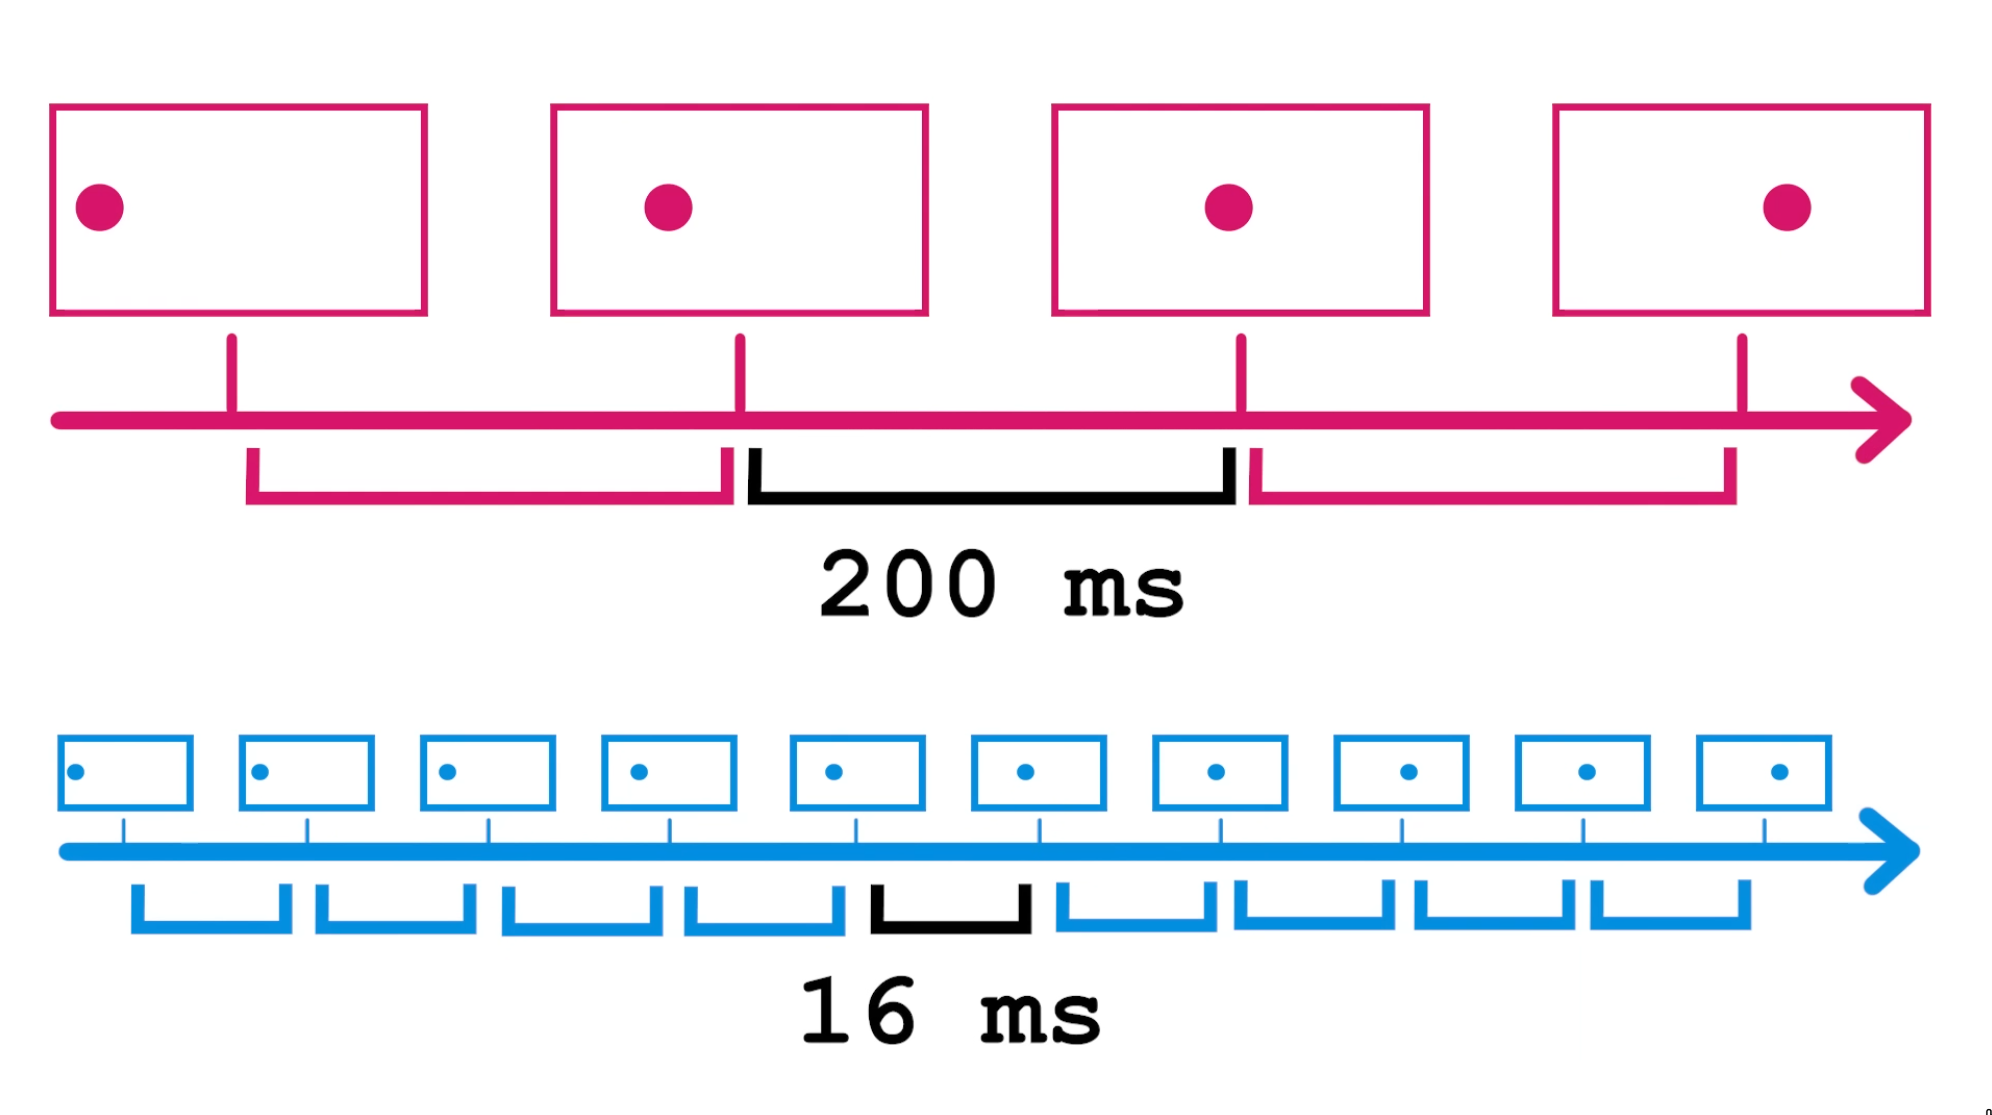
\includegraphics[width=0.8\textwidth]{time_between_frames.png}
    \caption{Time between frames displayed}
\end{figure}

\subsection{Potential problems}
A standard game loop runs one time each frame, before the frame is rendered.
The game loop is responsible for handling all the movement in the game, like moving the player.
If the game runs at 60FPS the game loop will be run 60 times each second.
\newline\newline
The following formula could be used to move the player each game loop iteration:
\newline
playerPosition.x = playerPosition.x + 10
\newline\newline
If this formula would be used to move the player, when running at 60PFS, the player would move 600 units of length each second.
But if the game was running at 30FPS, the player would only move 300 units each second.
So the player with 60FPS is considerably faster than the one with 30FPS.
This is of course, not ideal, as a game developer you want everyone to move at the same speed despite the computer it is run on.
The difference in elapsed distance is also shown in the figure below.
\begin{figure}[h!]
    \centering
    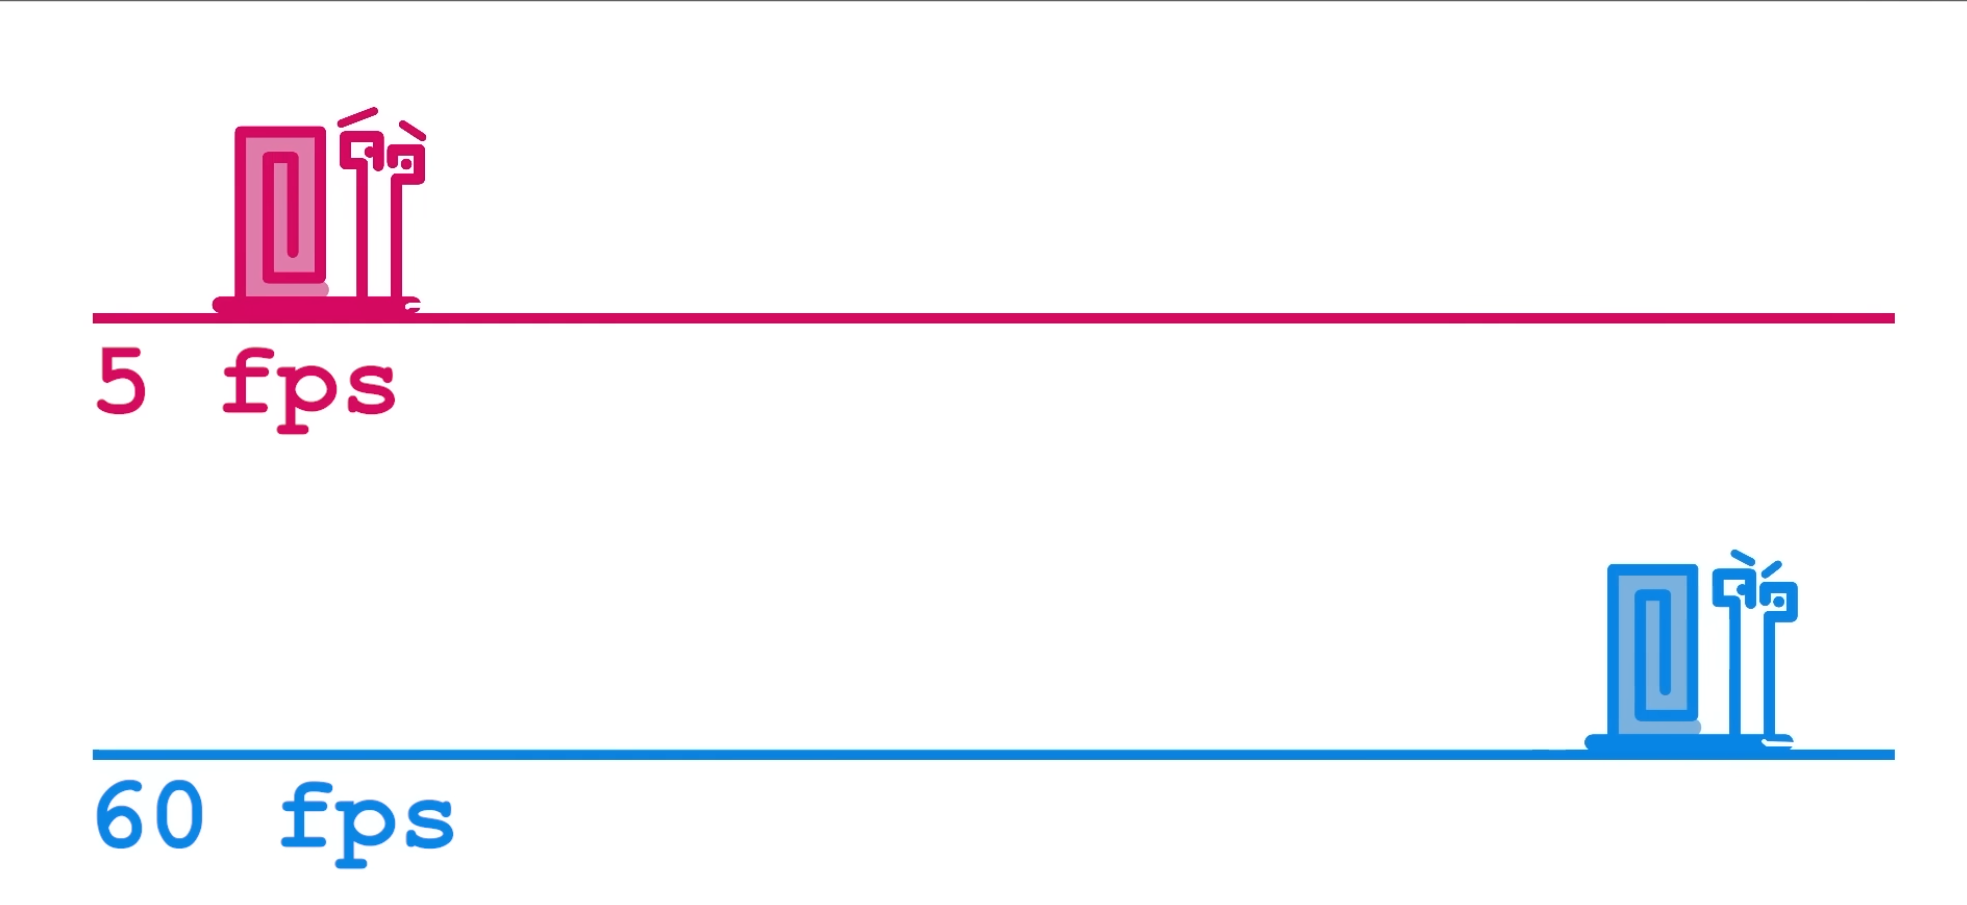
\includegraphics[width=0.8\textwidth]{difference_in_distance.png}
    \caption{Difference in elapsed distance}
\end{figure}

\subsection{Possible solutions}
There are two common solutions that help alleviate this problem, adjusting the movement speed relative to the FPS or making sure to handle movement in a fixed update loop that is guaranteed to run at a certain amount of cycles each second.

\subsubsection{Fixed update}
A solution to the differing movement speeds between computers, is to create a lightweight time based interrupt, often referred to as FixedUpdate, to handle all movement.
It is important that the FixedUpdate function is very small, otherwise the FixedUpdate could be too slow to be called at a constant rate each frame, defeating the purpose of the FixedUpdate.
In the figure below it is shown how times between different rendered frames can vary, while the FixedUpdate is called at a constant rate, where the small black bar represents the duration of the FixedUpdate function.
\begin{figure}[h!]
    \centering
    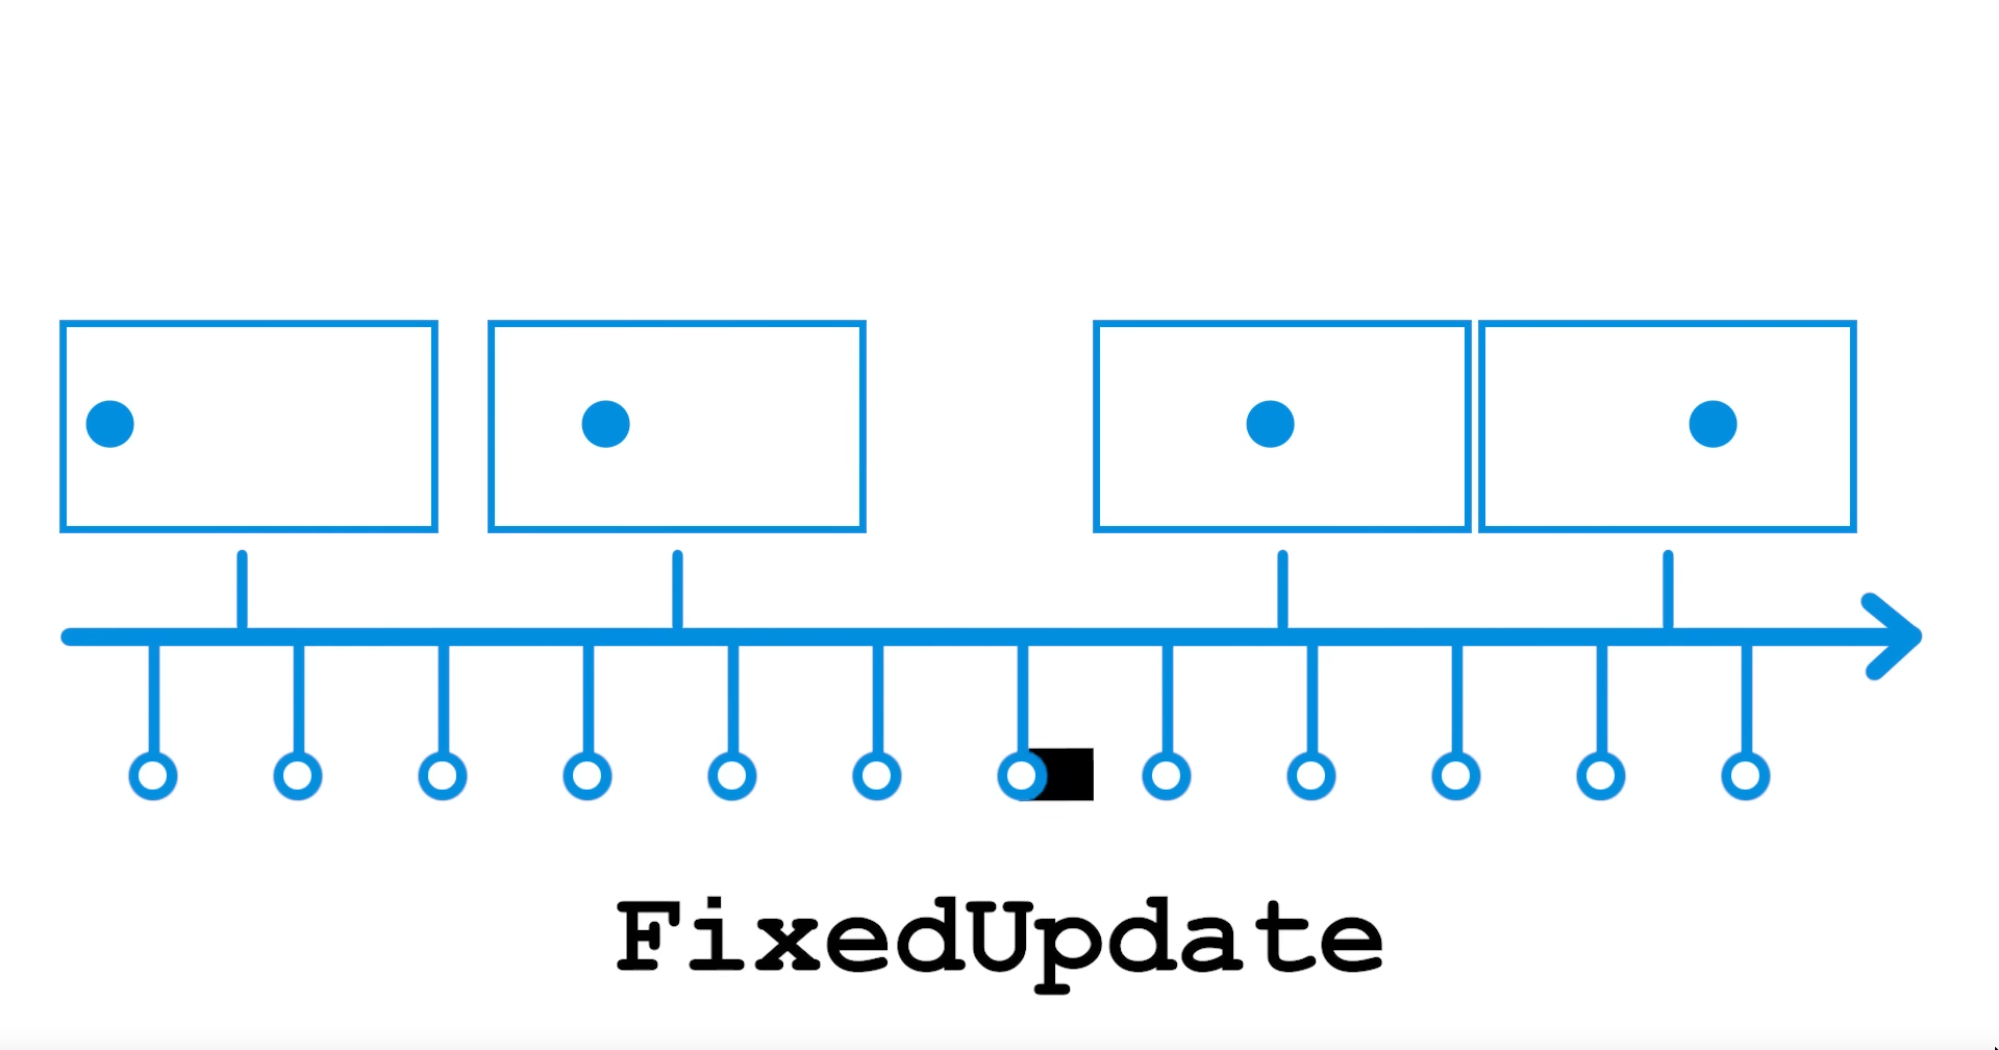
\includegraphics[width=0.6\textwidth]{fixed_update_explanation.png}
    \caption{Fixed update view}
\end{figure}
\subsubsection{Delta time}

\newpage
\section{sean}
\subsection{Multiplayer}
Whhich are frequently used multiplayer structures?
\subsection{input}
How do game engines handle input?
controller
\subsection{ai}
What kind of ai do game engines usually have?
pathfinding?
\newpage

\section{siem}
\subsection{audio}
How is audio played on linux?
multiple audio sources
directional audio
\subsection{save data}
What are common save data structures?
encryptie?
\newpage

\section{angel}
\subsection{particles}
What are particles in games?
What are common methods game engines use to render particles?
\subsection{physics}
What are physics in games?

common physics engines

\newpage

\section{ronan}
\subsection{levels}
What is a level in a video game?
How are transitions between levels done?
what are scenes?
How are levels saved/stored?
\subsection{gameobject}
What is a gameobject in a game engine?
How are components added to gameobjects?

\newpage

\section{temp}
bullet hell engine
\\
2d engine.
\\
wow factor: veel entiteiten op het scherm. gamepseed ver kunnen verogen.
performance tot de max.
\\
seger:
gamespeed
2d rendering
sprites (animatie + matrix berkeningen(rotere, schalen etc))
\\
sean:
Multiplayer
hoe connecten naar elkaar (ip adres, username?)
wie host? Central? peer to peer?
\\
input + controller support
ai
\\
siem:\\
audio + adaptive music\\
data opslaan (voortgang, levels, statistieken, unlocks, achievements, etc)\\
\\
angel:\\
particles?\\
physics\\
\\
ronan:\\
levels + levels switchen + scenes + hud \\
gameobject
\\

example of a reference \cite{author2020} like this test.


\newpage

\section{Bibliography}
\printbibliography %Prints bibliography
\newpage

\end{document} % This is the end of the document
